% Options for packages loaded elsewhere
\PassOptionsToPackage{unicode}{hyperref}
\PassOptionsToPackage{hyphens}{url}
\PassOptionsToPackage{dvipsnames,svgnames,x11names}{xcolor}
%
\documentclass[
  letterpaper,
  DIV=11,
  numbers=noendperiod]{scrartcl}

\usepackage{amsmath,amssymb}
\usepackage{lmodern}
\usepackage{iftex}
\ifPDFTeX
  \usepackage[T1]{fontenc}
  \usepackage[utf8]{inputenc}
  \usepackage{textcomp} % provide euro and other symbols
\else % if luatex or xetex
  \usepackage{unicode-math}
  \defaultfontfeatures{Scale=MatchLowercase}
  \defaultfontfeatures[\rmfamily]{Ligatures=TeX,Scale=1}
\fi
% Use upquote if available, for straight quotes in verbatim environments
\IfFileExists{upquote.sty}{\usepackage{upquote}}{}
\IfFileExists{microtype.sty}{% use microtype if available
  \usepackage[]{microtype}
  \UseMicrotypeSet[protrusion]{basicmath} % disable protrusion for tt fonts
}{}
\makeatletter
\@ifundefined{KOMAClassName}{% if non-KOMA class
  \IfFileExists{parskip.sty}{%
    \usepackage{parskip}
  }{% else
    \setlength{\parindent}{0pt}
    \setlength{\parskip}{6pt plus 2pt minus 1pt}}
}{% if KOMA class
  \KOMAoptions{parskip=half}}
\makeatother
\usepackage{xcolor}
\setlength{\emergencystretch}{3em} % prevent overfull lines
\setcounter{secnumdepth}{-\maxdimen} % remove section numbering
% Make \paragraph and \subparagraph free-standing
\ifx\paragraph\undefined\else
  \let\oldparagraph\paragraph
  \renewcommand{\paragraph}[1]{\oldparagraph{#1}\mbox{}}
\fi
\ifx\subparagraph\undefined\else
  \let\oldsubparagraph\subparagraph
  \renewcommand{\subparagraph}[1]{\oldsubparagraph{#1}\mbox{}}
\fi

\usepackage{color}
\usepackage{fancyvrb}
\newcommand{\VerbBar}{|}
\newcommand{\VERB}{\Verb[commandchars=\\\{\}]}
\DefineVerbatimEnvironment{Highlighting}{Verbatim}{commandchars=\\\{\}}
% Add ',fontsize=\small' for more characters per line
\usepackage{framed}
\definecolor{shadecolor}{RGB}{241,243,245}
\newenvironment{Shaded}{\begin{snugshade}}{\end{snugshade}}
\newcommand{\AlertTok}[1]{\textcolor[rgb]{0.68,0.00,0.00}{#1}}
\newcommand{\AnnotationTok}[1]{\textcolor[rgb]{0.37,0.37,0.37}{#1}}
\newcommand{\AttributeTok}[1]{\textcolor[rgb]{0.40,0.45,0.13}{#1}}
\newcommand{\BaseNTok}[1]{\textcolor[rgb]{0.68,0.00,0.00}{#1}}
\newcommand{\BuiltInTok}[1]{\textcolor[rgb]{0.00,0.23,0.31}{#1}}
\newcommand{\CharTok}[1]{\textcolor[rgb]{0.13,0.47,0.30}{#1}}
\newcommand{\CommentTok}[1]{\textcolor[rgb]{0.37,0.37,0.37}{#1}}
\newcommand{\CommentVarTok}[1]{\textcolor[rgb]{0.37,0.37,0.37}{\textit{#1}}}
\newcommand{\ConstantTok}[1]{\textcolor[rgb]{0.56,0.35,0.01}{#1}}
\newcommand{\ControlFlowTok}[1]{\textcolor[rgb]{0.00,0.23,0.31}{#1}}
\newcommand{\DataTypeTok}[1]{\textcolor[rgb]{0.68,0.00,0.00}{#1}}
\newcommand{\DecValTok}[1]{\textcolor[rgb]{0.68,0.00,0.00}{#1}}
\newcommand{\DocumentationTok}[1]{\textcolor[rgb]{0.37,0.37,0.37}{\textit{#1}}}
\newcommand{\ErrorTok}[1]{\textcolor[rgb]{0.68,0.00,0.00}{#1}}
\newcommand{\ExtensionTok}[1]{\textcolor[rgb]{0.00,0.23,0.31}{#1}}
\newcommand{\FloatTok}[1]{\textcolor[rgb]{0.68,0.00,0.00}{#1}}
\newcommand{\FunctionTok}[1]{\textcolor[rgb]{0.28,0.35,0.67}{#1}}
\newcommand{\ImportTok}[1]{\textcolor[rgb]{0.00,0.46,0.62}{#1}}
\newcommand{\InformationTok}[1]{\textcolor[rgb]{0.37,0.37,0.37}{#1}}
\newcommand{\KeywordTok}[1]{\textcolor[rgb]{0.00,0.23,0.31}{#1}}
\newcommand{\NormalTok}[1]{\textcolor[rgb]{0.00,0.23,0.31}{#1}}
\newcommand{\OperatorTok}[1]{\textcolor[rgb]{0.37,0.37,0.37}{#1}}
\newcommand{\OtherTok}[1]{\textcolor[rgb]{0.00,0.23,0.31}{#1}}
\newcommand{\PreprocessorTok}[1]{\textcolor[rgb]{0.68,0.00,0.00}{#1}}
\newcommand{\RegionMarkerTok}[1]{\textcolor[rgb]{0.00,0.23,0.31}{#1}}
\newcommand{\SpecialCharTok}[1]{\textcolor[rgb]{0.37,0.37,0.37}{#1}}
\newcommand{\SpecialStringTok}[1]{\textcolor[rgb]{0.13,0.47,0.30}{#1}}
\newcommand{\StringTok}[1]{\textcolor[rgb]{0.13,0.47,0.30}{#1}}
\newcommand{\VariableTok}[1]{\textcolor[rgb]{0.07,0.07,0.07}{#1}}
\newcommand{\VerbatimStringTok}[1]{\textcolor[rgb]{0.13,0.47,0.30}{#1}}
\newcommand{\WarningTok}[1]{\textcolor[rgb]{0.37,0.37,0.37}{\textit{#1}}}

\providecommand{\tightlist}{%
  \setlength{\itemsep}{0pt}\setlength{\parskip}{0pt}}\usepackage{longtable,booktabs,array}
\usepackage{calc} % for calculating minipage widths
% Correct order of tables after \paragraph or \subparagraph
\usepackage{etoolbox}
\makeatletter
\patchcmd\longtable{\par}{\if@noskipsec\mbox{}\fi\par}{}{}
\makeatother
% Allow footnotes in longtable head/foot
\IfFileExists{footnotehyper.sty}{\usepackage{footnotehyper}}{\usepackage{footnote}}
\makesavenoteenv{longtable}
\usepackage{graphicx}
\makeatletter
\def\maxwidth{\ifdim\Gin@nat@width>\linewidth\linewidth\else\Gin@nat@width\fi}
\def\maxheight{\ifdim\Gin@nat@height>\textheight\textheight\else\Gin@nat@height\fi}
\makeatother
% Scale images if necessary, so that they will not overflow the page
% margins by default, and it is still possible to overwrite the defaults
% using explicit options in \includegraphics[width, height, ...]{}
\setkeys{Gin}{width=\maxwidth,height=\maxheight,keepaspectratio}
% Set default figure placement to htbp
\makeatletter
\def\fps@figure{htbp}
\makeatother

\KOMAoption{captions}{tableheading}
\makeatletter
\makeatother
\makeatletter
\makeatother
\makeatletter
\@ifpackageloaded{caption}{}{\usepackage{caption}}
\AtBeginDocument{%
\ifdefined\contentsname
  \renewcommand*\contentsname{Table of contents}
\else
  \newcommand\contentsname{Table of contents}
\fi
\ifdefined\listfigurename
  \renewcommand*\listfigurename{List of Figures}
\else
  \newcommand\listfigurename{List of Figures}
\fi
\ifdefined\listtablename
  \renewcommand*\listtablename{List of Tables}
\else
  \newcommand\listtablename{List of Tables}
\fi
\ifdefined\figurename
  \renewcommand*\figurename{Figure}
\else
  \newcommand\figurename{Figure}
\fi
\ifdefined\tablename
  \renewcommand*\tablename{Table}
\else
  \newcommand\tablename{Table}
\fi
}
\@ifpackageloaded{float}{}{\usepackage{float}}
\floatstyle{ruled}
\@ifundefined{c@chapter}{\newfloat{codelisting}{h}{lop}}{\newfloat{codelisting}{h}{lop}[chapter]}
\floatname{codelisting}{Listing}
\newcommand*\listoflistings{\listof{codelisting}{List of Listings}}
\makeatother
\makeatletter
\@ifpackageloaded{caption}{}{\usepackage{caption}}
\@ifpackageloaded{subcaption}{}{\usepackage{subcaption}}
\makeatother
\makeatletter
\@ifpackageloaded{tcolorbox}{}{\usepackage[many]{tcolorbox}}
\makeatother
\makeatletter
\@ifundefined{shadecolor}{\definecolor{shadecolor}{rgb}{.97, .97, .97}}
\makeatother
\makeatletter
\makeatother
\ifLuaTeX
  \usepackage{selnolig}  % disable illegal ligatures
\fi
\IfFileExists{bookmark.sty}{\usepackage{bookmark}}{\usepackage{hyperref}}
\IfFileExists{xurl.sty}{\usepackage{xurl}}{} % add URL line breaks if available
\urlstyle{same} % disable monospaced font for URLs
\hypersetup{
  pdftitle={Simulation Withing},
  pdfauthor={Federico Maioli},
  colorlinks=true,
  linkcolor={blue},
  filecolor={Maroon},
  citecolor={Blue},
  urlcolor={Blue},
  pdfcreator={LaTeX via pandoc}}

\title{Simulation Withing}
\author{Federico Maioli}
\date{}

\begin{document}
\maketitle
\ifdefined\Shaded\renewenvironment{Shaded}{\begin{tcolorbox}[enhanced, borderline west={3pt}{0pt}{shadecolor}, sharp corners, boxrule=0pt, interior hidden, breakable, frame hidden]}{\end{tcolorbox}}\fi

\hypertarget{load-the-libraries}{%
\subsection{Load the libraries}\label{load-the-libraries}}

\begin{Shaded}
\begin{Highlighting}[]
\FunctionTok{library}\NormalTok{(tidyverse)}
\end{Highlighting}
\end{Shaded}

\begin{verbatim}
-- Attaching core tidyverse packages ------------------------ tidyverse 2.0.0 --
v dplyr     1.1.2     v readr     2.1.4
v forcats   1.0.0     v stringr   1.5.0
v ggplot2   3.4.2     v tibble    3.2.1
v lubridate 1.9.2     v tidyr     1.3.0
v purrr     1.0.1     
-- Conflicts ------------------------------------------ tidyverse_conflicts() --
x dplyr::filter() masks stats::filter()
x dplyr::lag()    masks stats::lag()
i Use the ]8;;http://conflicted.r-lib.org/conflicted package]8;; to force all conflicts to become errors
\end{verbatim}

\begin{Shaded}
\begin{Highlighting}[]
\FunctionTok{library}\NormalTok{(sdmTMB)}
\end{Highlighting}
\end{Shaded}

\hypertarget{simulate-the-dataset}{%
\subsection{Simulate the dataset}\label{simulate-the-dataset}}

\begin{Shaded}
\begin{Highlighting}[]
\FunctionTok{set.seed}\NormalTok{(}\DecValTok{99}\NormalTok{)}

\CommentTok{\# true data}
\NormalTok{true\_data }\OtherTok{\textless{}{-}} \FunctionTok{data.frame}\NormalTok{(}
  \AttributeTok{X =} \FunctionTok{runif}\NormalTok{(}\DecValTok{1000}\NormalTok{), }\AttributeTok{Y =} \FunctionTok{runif}\NormalTok{(}\DecValTok{1000}\NormalTok{), }\CommentTok{\# coordinates}
  \AttributeTok{b1 =} \FunctionTok{rnorm}\NormalTok{(}\DecValTok{1000}\NormalTok{), }\AttributeTok{b2 =} \FunctionTok{rnorm}\NormalTok{(}\DecValTok{1000}\NormalTok{), }\CommentTok{\# beta1 and beta 2}
  \AttributeTok{year =} \FunctionTok{rep}\NormalTok{(}\DecValTok{1}\SpecialCharTok{:}\DecValTok{20}\NormalTok{, }\AttributeTok{each =} \DecValTok{50}\NormalTok{),}
  \AttributeTok{f\_year =} \FunctionTok{as.factor}\NormalTok{(}\FunctionTok{rep}\NormalTok{(}\DecValTok{1}\SpecialCharTok{:}\DecValTok{20}\NormalTok{, }\AttributeTok{each =} \DecValTok{50}\NormalTok{)) }\CommentTok{\# for random intercept}
\NormalTok{)}

\CommentTok{\# mesh}
\NormalTok{true\_mesh }\OtherTok{\textless{}{-}} \FunctionTok{make\_mesh}\NormalTok{(true\_data, }\AttributeTok{xy\_cols =} \FunctionTok{c}\NormalTok{(}\StringTok{"X"}\NormalTok{, }\StringTok{"Y"}\NormalTok{), }\AttributeTok{type=}\StringTok{\textquotesingle{}kmeans\textquotesingle{}}\NormalTok{,}\AttributeTok{n\_knots =} \DecValTok{300}\NormalTok{)}
\end{Highlighting}
\end{Shaded}

\begin{verbatim}
as(<dgCMatrix>, "dgTMatrix") is deprecated since Matrix 1.5-0; do as(., "TsparseMatrix") instead
\end{verbatim}

\begin{Shaded}
\begin{Highlighting}[]
\FunctionTok{plot}\NormalTok{(true\_mesh)}
\end{Highlighting}
\end{Shaded}

\begin{figure}[H]

{\centering 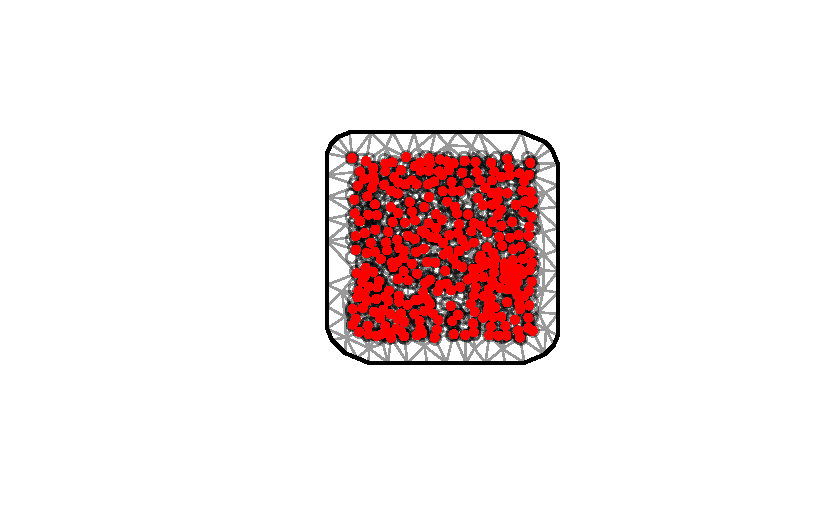
\includegraphics{simulation_sdmTMB_files/figure-pdf/unnamed-chunk-2-1.pdf}

}

\end{figure}

\begin{Shaded}
\begin{Highlighting}[]
\CommentTok{\# data{-}generating model}
\NormalTok{sim\_data }\OtherTok{\textless{}{-}} \FunctionTok{sdmTMB\_simulate}\NormalTok{(}
  \AttributeTok{formula =} \SpecialCharTok{\textasciitilde{}} \DecValTok{1} \SpecialCharTok{+}\NormalTok{ b1 }\SpecialCharTok{+}\NormalTok{ b2 }\SpecialCharTok{+}\NormalTok{ (}\DecValTok{1}\SpecialCharTok{|}\NormalTok{f\_year), }\CommentTok{\# data generating formula}
  \AttributeTok{data =}\NormalTok{ true\_data,}
  \AttributeTok{time =} \StringTok{"year"}\NormalTok{,}
  \AttributeTok{mesh =}\NormalTok{ true\_mesh,}
  \AttributeTok{family =} \FunctionTok{tweedie}\NormalTok{(),}
  \AttributeTok{range =} \FloatTok{0.5}\NormalTok{, }\CommentTok{\# true matern range}
  \AttributeTok{sigma\_O =} \FloatTok{0.7}\NormalTok{, }\CommentTok{\# true spatial sd}
  \AttributeTok{phi =} \FloatTok{0.9}\NormalTok{, }\CommentTok{\# the tweedie param}
  \AttributeTok{B =} \FunctionTok{c}\NormalTok{(}\FloatTok{0.2}\NormalTok{, }\SpecialCharTok{{-}}\FloatTok{0.4}\NormalTok{, }\FloatTok{0.3}\NormalTok{) }\CommentTok{\# true betas}
\NormalTok{)}
\CommentTok{\# see https://pbs{-}assess.github.io/sdmTMB/ for synatx details}

\NormalTok{sim\_data}\SpecialCharTok{$}\NormalTok{f\_year }\OtherTok{\textless{}{-}} \FunctionTok{as.factor}\NormalTok{(sim\_data}\SpecialCharTok{$}\NormalTok{year)}
\end{Highlighting}
\end{Shaded}

\hypertarget{we-now-fit-the-model-with-the-full-data}{%
\subsection{We now fit the model with the full
data}\label{we-now-fit-the-model-with-the-full-data}}

\begin{Shaded}
\begin{Highlighting}[]
\CommentTok{\# first a mesh}
\NormalTok{mesh\_full }\OtherTok{\textless{}{-}} \FunctionTok{make\_mesh}\NormalTok{(sim\_data, }\AttributeTok{xy\_cols =} \FunctionTok{c}\NormalTok{(}\StringTok{"X"}\NormalTok{, }\StringTok{"Y"}\NormalTok{), }\AttributeTok{type=}\StringTok{\textquotesingle{}kmeans\textquotesingle{}}\NormalTok{,}\AttributeTok{n\_knots =} \DecValTok{300}\NormalTok{)}
\FunctionTok{plot}\NormalTok{(mesh\_full)}
\end{Highlighting}
\end{Shaded}

\begin{figure}[H]

{\centering 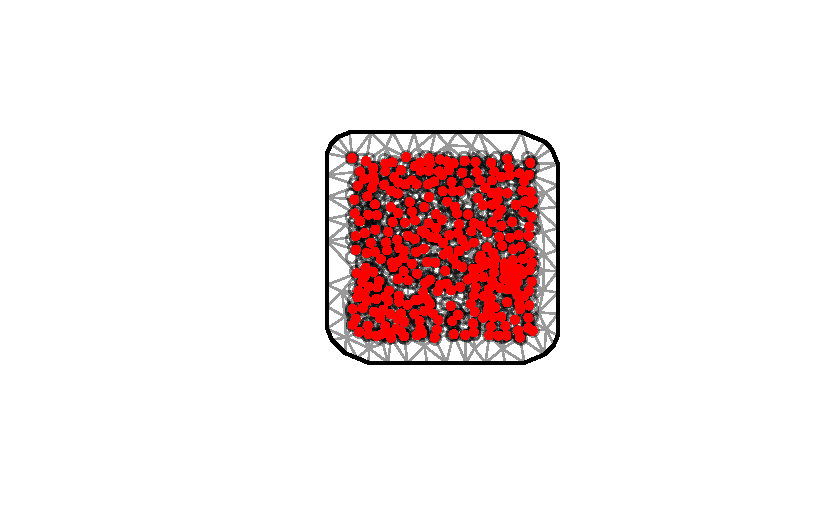
\includegraphics{simulation_sdmTMB_files/figure-pdf/unnamed-chunk-3-1.pdf}

}

\end{figure}

\begin{Shaded}
\begin{Highlighting}[]
\CommentTok{\# now the model}
\NormalTok{m\_full}\OtherTok{=}\FunctionTok{sdmTMB}\NormalTok{(observed }\SpecialCharTok{\textasciitilde{}} \DecValTok{1} \SpecialCharTok{+}\NormalTok{ b1 }\SpecialCharTok{+}\NormalTok{ b2 }\SpecialCharTok{+}\NormalTok{ (}\DecValTok{1}\SpecialCharTok{|}\NormalTok{f\_year),}
              \AttributeTok{data =}\NormalTok{ sim\_data, }\AttributeTok{mesh =}\NormalTok{ mesh\_full, }\AttributeTok{time =} \StringTok{"year"}\NormalTok{,}\AttributeTok{spatiotemporal =} \StringTok{\textquotesingle{}off\textquotesingle{}}\NormalTok{,}
              \AttributeTok{family =} \FunctionTok{tweedie}\NormalTok{())}

\FunctionTok{summary}\NormalTok{(m\_full)}
\end{Highlighting}
\end{Shaded}

\begin{verbatim}
Spatial model fit by ML ['sdmTMB']
Formula: observed ~ 1 + b1 + b2 + (1 | f_year)
Mesh: mesh_full
Time column: year
Data: sim_data
Family: tweedie(link = 'log')
 
            coef.est coef.se
(Intercept)     0.54    0.30
b1             -0.37    0.03
b2              0.29    0.03

Random intercepts:
       Std. Dev.
f_year      1.02

Dispersion parameter: 0.93
Tweedie p: 1.50
Matern range: 0.36
Spatial SD: 0.52
ML criterion at convergence: 1840.409

See ?tidy.sdmTMB to extract these values as a data frame.
\end{verbatim}

\hypertarget{we-remove-some-data}{%
\subsection{We remove some data}\label{we-remove-some-data}}

Here we remove for 3 years (year 1,5, and 15) the values of the
coordinates X \textless{} 0.6. This is somehow similar to the case of
the withing paper. We lose 10\% of the hauls.

\begin{Shaded}
\begin{Highlighting}[]
\NormalTok{sim\_data\_missing}\OtherTok{=}\NormalTok{sim\_data }\SpecialCharTok{\%\textgreater{}\%} \FunctionTok{filter}\NormalTok{(}\SpecialCharTok{!}\NormalTok{(X}\SpecialCharTok{\textless{}}\FloatTok{0.6} \SpecialCharTok{\&}\NormalTok{ year}\SpecialCharTok{==}\DecValTok{1}\NormalTok{) }\SpecialCharTok{\&} \SpecialCharTok{!}\NormalTok{(X}\SpecialCharTok{\textless{}}\FloatTok{0.6} \SpecialCharTok{\&}\NormalTok{ year}\SpecialCharTok{==}\DecValTok{15}\NormalTok{) }\SpecialCharTok{\&} \SpecialCharTok{!}\NormalTok{(X}\SpecialCharTok{\textless{}}\FloatTok{0.6} \SpecialCharTok{\&}\NormalTok{ year}\SpecialCharTok{==}\DecValTok{5}\NormalTok{))}
\end{Highlighting}
\end{Shaded}

\hypertarget{we-refit-the-model-using-the-dataset-with-the-missing-values}{%
\subsection{We refit the model using the dataset with the missing
values}\label{we-refit-the-model-using-the-dataset-with-the-missing-values}}

\begin{Shaded}
\begin{Highlighting}[]
\CommentTok{\# first a mesh}
\NormalTok{mesh\_missing }\OtherTok{\textless{}{-}} \FunctionTok{make\_mesh}\NormalTok{(sim\_data\_missing, }\AttributeTok{xy\_cols =} \FunctionTok{c}\NormalTok{(}\StringTok{"X"}\NormalTok{, }\StringTok{"Y"}\NormalTok{), }\AttributeTok{type=}\StringTok{\textquotesingle{}kmeans\textquotesingle{}}\NormalTok{,}\AttributeTok{n\_knots =} \DecValTok{300}\NormalTok{)}
\FunctionTok{plot}\NormalTok{(mesh\_missing)}
\end{Highlighting}
\end{Shaded}

\begin{figure}[H]

{\centering 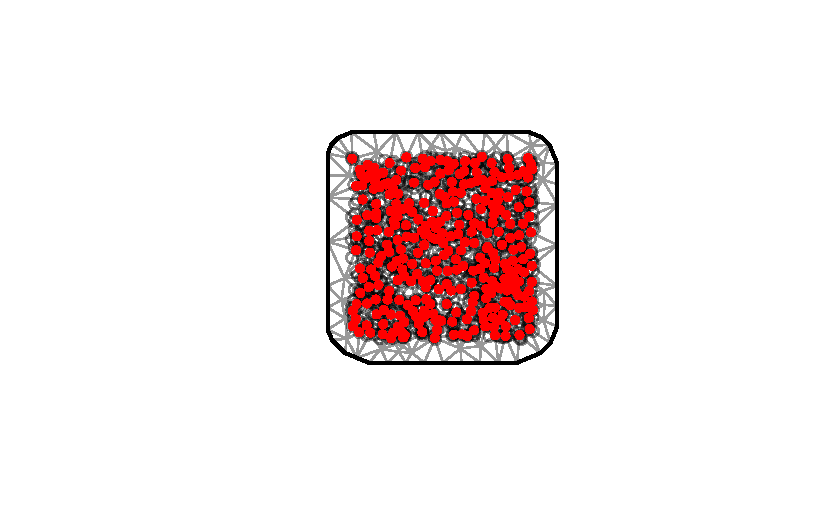
\includegraphics{simulation_sdmTMB_files/figure-pdf/unnamed-chunk-5-1.pdf}

}

\end{figure}

\begin{Shaded}
\begin{Highlighting}[]
\CommentTok{\# now the model}
\NormalTok{m\_missing}\OtherTok{=}\FunctionTok{sdmTMB}\NormalTok{(observed }\SpecialCharTok{\textasciitilde{}} \DecValTok{1} \SpecialCharTok{+}\NormalTok{ b1 }\SpecialCharTok{+}\NormalTok{ b2 }\SpecialCharTok{+}\NormalTok{ (}\DecValTok{1}\SpecialCharTok{|}\NormalTok{f\_year),}
              \AttributeTok{data =}\NormalTok{ sim\_data\_missing, }\AttributeTok{mesh =}\NormalTok{ mesh\_missing, }\AttributeTok{time =} \StringTok{"year"}\NormalTok{,}\AttributeTok{spatiotemporal =} \StringTok{\textquotesingle{}off\textquotesingle{}}\NormalTok{,}
              \AttributeTok{family =} \FunctionTok{tweedie}\NormalTok{())}

\FunctionTok{summary}\NormalTok{(m\_missing)}
\end{Highlighting}
\end{Shaded}

\begin{verbatim}
Spatial model fit by ML ['sdmTMB']
Formula: observed ~ 1 + b1 + b2 + (1 | f_year)
Mesh: mesh_missing
Time column: year
Data: sim_data_missing
Family: tweedie(link = 'log')
 
            coef.est coef.se
(Intercept)     0.55    0.31
b1             -0.37    0.03
b2              0.29    0.03

Random intercepts:
       Std. Dev.
f_year      1.03

Dispersion parameter: 0.93
Tweedie p: 1.51
Matern range: 0.39
Spatial SD: 0.51
ML criterion at convergence: 1656.657

See ?tidy.sdmTMB to extract these values as a data frame.
\end{verbatim}

\hypertarget{the-model-looks-quite-similar-lets-plot-them}{%
\subsection{The model looks quite similar, let's plot
them}\label{the-model-looks-quite-similar-lets-plot-them}}



\end{document}
